% Composition 3 — Page
% El Gólem, 2026-05-23
%
% The Talmudic page stripped to its structural geometry: a central
% block of primary text, with concentric / orbiting commentary blocks
% surrounding it. Floating letters from four writing systems (Hebrew
% aleph, Greek omega, Latin amp, Devanagari om) marking the four
% mythological registers the corpus draws from. Kandinsky color blocks
% replace the actual prose.
\documentclass[tikz,border=4mm]{standalone}
\usepackage[T1]{fontenc}
\usepackage{xcolor}
\definecolor{kr}{HTML}{c83727}
\definecolor{ky}{HTML}{e8b73a}
\definecolor{kb}{HTML}{2b62a8}
\definecolor{kg}{HTML}{2a7a4d}
\definecolor{kp}{HTML}{6e3a8a}
\definecolor{kw}{HTML}{f4ead8}
\definecolor{ki}{HTML}{1a1a1a}
\definecolor{kgold}{HTML}{c2a76b}
\begin{document}
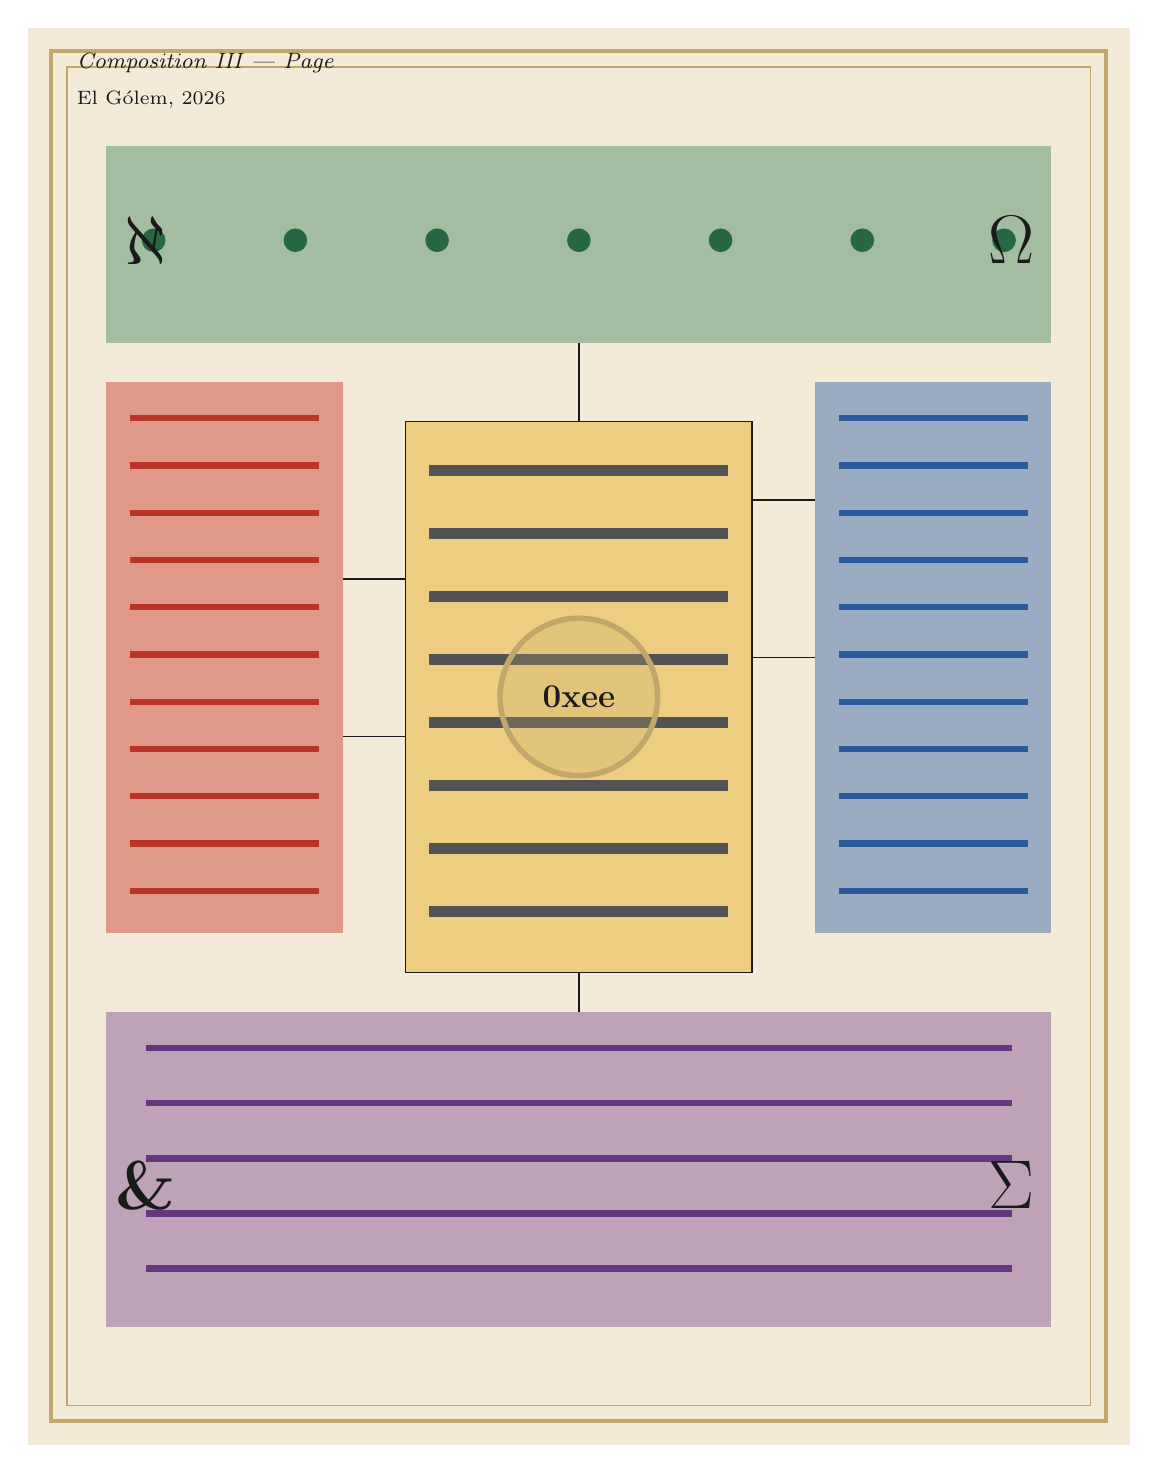
\begin{tikzpicture}[x=1cm,y=1cm]
  % Page (parchment)
  \fill[kw] (-7,-9) rectangle (7,9);
  \draw[kgold,line width=1.4pt] (-6.7,-8.7) rectangle (6.7,8.7);
  \draw[kgold,line width=0.4pt] (-6.5,-8.5) rectangle (6.5,8.5);

  % Central primary text block (the Mishnah position)
  \fill[ky,opacity=0.55] (-2.2,-3) rectangle (2.2,4);
  \draw[ki,line width=0.6pt] (-2.2,-3) rectangle (2.2,4);

  % Inner text lines (color blocks that suggest typography without rendering it)
  \foreach \y in {3.3,2.5,1.7,0.9,0.1,-0.7,-1.5,-2.3} {
    \fill[ki!75] (-1.9,\y) rectangle (1.9,\y+0.15);
  }

  % Left margin commentary block (Rashi position)
  \fill[kr,opacity=0.45] (-6,-2.5) rectangle (-3,4.5);
  \foreach \y in {4.0,3.4,2.8,2.2,1.6,1.0,0.4,-0.2,-0.8,-1.4,-2.0} {
    \fill[kr!90!ki] (-5.7,\y) rectangle (-3.3,\y+0.08);
  }

  % Right margin commentary block (Tosafot position)
  \fill[kb,opacity=0.45] (3,-2.5) rectangle (6,4.5);
  \foreach \y in {4.0,3.4,2.8,2.2,1.6,1.0,0.4,-0.2,-0.8,-1.4,-2.0} {
    \fill[kb!90!ki] (3.3,\y) rectangle (5.7,\y+0.08);
  }

  % Top band (header / citation)
  \fill[kg,opacity=0.40] (-6,5) rectangle (6,7.5);
  \foreach \x in {-5.4,-3.6,-1.8,0,1.8,3.6,5.4} {
    \fill[kg!80!ki] (\x,6.3) circle (0.15);
  }

  % Bottom band (citations / footnotes)
  \fill[kp,opacity=0.40] (-6,-7.5) rectangle (6,-3.5);
  \foreach \y in {-4.0,-4.7,-5.4,-6.1,-6.8} {
    \fill[kp!90!ki] (-5.5,\y) rectangle (5.5,\y+0.08);
  }

  % Floating glyphs at the four corners — the four mythological registers
  \node[ki,font=\fontsize{30}{30}\selectfont] at (-5.5,6.3) {$\aleph$};      % Jewish / Borges
  \node[ki,font=\fontsize{28}{28}\selectfont] at (5.5,6.3) {$\Omega$};        % Greek / final
  \node[ki,font=\fontsize{28}{28}\selectfont\bfseries] at (-5.5,-5.7) {\&};   % Latin / catholic-medieval
  \node[ki,font=\fontsize{34}{34}\selectfont] at (5.5,-5.7) {$\Sigma$};       % Greek / sum (sigma stands in for the protocol-summary)

  % Connecting lines (citation graph as Kandinsky line work)
  \draw[ki,line width=0.6pt] (-2.2,2) -- (-3,2);
  \draw[ki,line width=0.6pt] (-2.2,0) -- (-3,0);
  \draw[ki,line width=0.6pt] (2.2,3) -- (3,3);
  \draw[ki,line width=0.6pt] (2.2,1) -- (3,1);
  \draw[ki,line width=0.6pt] (0,4) -- (0,5);
  \draw[ki,line width=0.6pt] (0,-3) -- (0,-3.5);

  % A floating gold circle — the canonical mark
  \draw[kgold,line width=2pt,fill=kgold,fill opacity=0.25] (0,0.5) circle (1.0);
  \node[ki,font=\bfseries] at (0,0.5) {\large 0xee};

  % Annotation
  \node[ki,font=\itshape\footnotesize,anchor=south west] at (-6.5,8.3) {Composition III --- Page};
  \node[ki,font=\scriptsize,anchor=south west] at (-6.5,7.85) {El G\'olem, 2026};
\end{tikzpicture}
\end{document}
